% !TEX TS-program = pdflatex
% !TEX encoding = UTF-8 Unicode

% This is a simple template for a LaTeX document using the "article" class.
% See "book", "report", "letter" for other types of document.

%%%%%%%%%%%%%%%%%%%%%%%%%%%%%%%%%%%%%
%
% Template para producir documentos "camera ready" para Anales de la AFA
% 
%  No se debería tener que modificar nada del siguiente preámbulo, donde están 
%  las customizaciones para adaptar la clase "article" a los Anales AFA.
%
%%%%%%%%%%%%%%%%%%%%%%%%%%%%%%%%%%%%%
\documentclass[10pt,twocolumn]{article} 

\usepackage[utf8]{inputenc} % set input encoding (not needed with XeLaTeX)
\usepackage[spanish]{babel}


%%% DIMENSIONES DE LA PÁGINA
\usepackage{geometry} 
\geometry{a4paper} 
 \geometry{top=2.25cm} 
 \geometry{bottom=2.25cm} 
 \geometry{left=2.5cm} 
 \geometry{right=2cm} 


%%% PACKAGES
\usepackage{graphicx} 
\usepackage{paralist} % very flexible & customisable lists (eg. enumerate/itemize, etc.)
\usepackage{verbatim} % adds environment for commenting out blocks of text & for better verbatim
\usepackage{subfig} % make it possible to include more than one captioned figure/table in a single float
\usepackage{lipsum}  
\usepackage{hyperref}
\usepackage[superscript]{cite}  %REFERENCIAS EN SUPERÍNDICE

% Ajusta los captions de tablas y figuras a italics
\usepackage[format=plain,
            labelfont=it,
            textfont=it]{caption}
% These packages are all incorporated in the memoir class to one degree or another...

%%% HEADERS & FOOTERS
\usepackage{fancyhdr} % This should be set AFTER setting up the page geometry
\pagestyle{fancy} % options: empty , plain , fancy
\renewcommand{\headrulewidth}{0pt} % customise the layout...
\lhead{}\chead{}\rhead{}
\lfoot{}\cfoot{\thepage}\rfoot{}
%\renewcommand{\thefootnote}{\fnsymbol{footnote}}

\usepackage{varwidth}
\usepackage{authblk}
\newcommand{\filiacion}[2]{\affil[#1]{\protect\begin{varwidth}[t]{\linewidth}\protect\centering \normalfont#2 \protect\end{varwidth}}}
\newcommand{\autor}[2]{\author[#1]{\bf #2}}
\newcommand{\corresponding}[2]{\author[#1]{\bf #2}}
\newcommand\cauthemail[1]{\thanks{#1}}
\newcommand{\fecha}[1]{\date{\vspace{-1ex}\small{#1}}}
\newcommand{\titulo}[2]{\title{\bf{\large{#1 \\ \vspace{1.5ex} #2 }}}}
\newcommand{\esresumen}[1]{\small{#1 \par}\vspace{1.5ex}}
\newcommand{\pclaves}[1]{\small{\emph{#1} \par}\vspace{1.5ex}}
\newcommand{\enresumen}[1]{\small{#1 \par}\vspace{1.5ex}}
\newcommand{\keywords}[1]{\small{\emph{#1} \par}\vspace{1.5ex}}

%% otro paquete que agrego yo
\usepackage{amsmath}
%%

%%% APARIENCIA DE TITULOS, SECCIONES Y SUBSECCIONES
\usepackage{sectsty}
\allsectionsfont{\fontsize{10}{12}\sffamily\bfseries\upshape} % (See the fntguide.pdf for font help)

\usepackage{titlesec}
\titlespacing*{\section}{0pt}{1.5ex}{0.8ex}
\titlespacing*{\subsection}{0pt}{1.2ex}{0.6ex}
\setcounter{secnumdepth}{0}   %no numera las subsecciones

\usepackage[nottoc,notlof,notlot]{tocbibind} % Put the bibliography in the ToC
\usepackage[titles,subfigure]{tocloft} % Alter the style of the Table of Contents
\renewcommand{\cftsecfont}{\rmfamily\mdseries\upshape}
\renewcommand{\cftsecpagefont}{\rmfamily\mdseries\upshape} % No bold!
\renewcommand\thesection{\Roman{section}}
\renewcommand\thesubsection{}


%agregado
%\renewcommand\theHsubsection{\thesection.\arabic{subsection}}
%%


%%% PARA EL FORMATO DE TABLAS
\usepackage{booktabs} % for much better looking tables
\usepackage{array} % for better arrays (eg matrices) in maths
\makeatletter
\newcommand{\thickhline}{%
    \noalign {\ifnum 0=`}\fi \hrule height 1.5pt
    \futurelet \reserved@a \@xhline
}
\newcolumntype{"}{@{\hskip\tabcolsep\vrule width 1pt\hskip\tabcolsep}}
\makeatother
\newcolumntype{L}[1]{>{\raggedright\let\newline\\\arraybackslash\hspace{0pt}}m{#1}}
\newcolumntype{C}[1]{>{\centering\let\newline\\\arraybackslash\hspace{0pt}}m{#1}}
\newcolumntype{R}[1]{>{\raggedleft\let\newline\\\arraybackslash\hspace{0pt}}m{#1}}

\renewcommand\spanishtablename{Tabla}  

% Corresponding author
\makeatletter
\renewcommand\@biblabel[1]{#1.}
\makeatother

\pagestyle{empty}

%%%%%% En principio no debería hacer falta modificar nada por encima de esta línea

%%%%%%%%%%%%%%%%%%%%%%%%%%%%%%%%%%%%%%%

%%% El contenido del documento comienza a partir de acá 

%título del trabajo: en el primer campo en castellano, en el segundo en inglés
\titulo{CURVA CARACTERÍSTICA DE DIODO}
 
\autor{ }{César Orlando Solis \\ \small \texttt{cesar.solis@mi.unc.edu.ar}}

%\text{ \href{mailto:cesar.solis@mi.unc.edu.ar}{cesar.solis@mi.unc.edu.ar}}
%\autor{ }{Y.Y. Beta}
%\corresponding{1,2}{Z.Z. Gamma} %corresponding author 


%afiliaciones: se pueden combinar% Facultad de Matematica, Astronomia, Fisica y Computacion, UNC - Av. Medina Allende - (5000) Cordoba - Argentina
\filiacion{ }{Facultad de Matematica, Astronomia, Fisica y Computacion, UNC\par
Av. Medina Allende - (5000) Córdoba – Argentina}
%\filiacion{2}{Centro de Investigaciones en Láseres y Aplicaciones  CEILAP (CITEDEF-CONICET)
%J. B. de La Salle 4397 \par (B1603ALO) Villa Martelli – Prov. Buenos Aires – Argentina}

\fecha{Fecha: 13/05/26 }%;Aceptado: xx/xx/xx} %No modificar


\setcounter{Maxaffil}{0}
\renewcommand\Affilfont{\itshape\small}


\begin{document}

\renewcommand{\abstractname}{}
\twocolumn[
  \begin{@twocolumnfalse}
   \maketitle
    \begin{abstract}\vspace{-12ex}
\centering\begin{minipage}{\dimexpr\paperwidth-6cm}

%Abstract en castellano
\esresumen{%En este trabajo se analiza la curva caracteristica de un diodo conectado en serie con resistencias, y mediante ajuste no lineal se determina la corriente de 
%saturacion y el material con el que está fabricado, determinando que está fabricado de silicio. 

En este trabajo se analiza la curva característica de un diodo conectado en serie con resistencias.
 Mediante un ajuste no lineal utilizando la ecuación de Shockley, se determinó la corriente de saturación 
 $I_S = (1,0 \pm 0,1) \times 10^{-8}\text{ A}$ y el coeficiente $\eta = (1,71 \pm 0,01)$ , confirmando 
que el componente está fabricado de silicio. Si bien los parámetros concuerdan con los rangos teóricos esperados
, el análisis de los residuos del ajuste indica que el modelo ideal no describe completamente el comportamiento del diodo, 
sugiriendo la necesidad de considerar otros factores para mejorarlo.

}
%\pclaves{Palabras Clave: preparación, manuscritos, publicación.} %palabras clave

%Abstract en inglés
%\enresumen{In this paper the instructions for making “camera-ready” contributions to ANALES AFA are presented. This document can be found via Internet in the home pages of the Universidad Nacional de San Luis, under the appropiate choice.}
%\keywords{Keywords: making, papers, publishing.}  %key words

\end{minipage}
\vspace{4ex}
 \end{abstract}
  \end{@twocolumnfalse}
]

\thispagestyle{empty}

\setcounter{footnote}{1}
%\begin{equation} \end{equation}
%
\section{INTRODUCCIÓN}
El diodo es un dispositivo electrónico formado por la unión de dos materiales semiconductores, uno tipo p (ánodo) y otro tipo n (cátodo), que permite el paso de corriente en un solo sentido.
En un diodo, la relación entre la corriente $I$ y el voltaje $V$ se describe por la ecuación de Shockley, dada por:
\begin{equation}I_D=I_S \left[e^{V_D/(\eta V_T)}-1\right]\end{equation}
Donde $I_S$ es la corriente de saturación, $\eta$ es el coeficiente de emisión, que depende del material con que esta fabricado el diodo, y $V_T$ es la tensión equivalente de temperatura,
que cumple:
\begin{equation}V_T = kT/q\end{equation}
 Con la temperatura $T$ en Kelvin.


 Cuando el diodo esta conectado en polarización directa, permitiendo el paso de corriente, con una resistencia en serie, como se puede ver en la figura(1), usando la ley de Ohm y las leyes de Kirchhoff, se llega a la siguiente relación: $V_{CC}=V_D +I_DR $ , donde $V_{CC}$ es el voltaje de la fuente, $R$ es la resistencia en serie, $V_D$ es la tensión en el diodo e $I_D$ es la corriente que circula por el circuito.
De modo que se puede escribir la corriente $I_D$ en función de la tensión $V_D$ en el diodo:
\begin{equation} I_D=\left(\frac{-1}{R}\right)V_D+\frac{V_{CC}}{R}\end{equation}
 %
    \begin{figure}[ht]
    \centering
    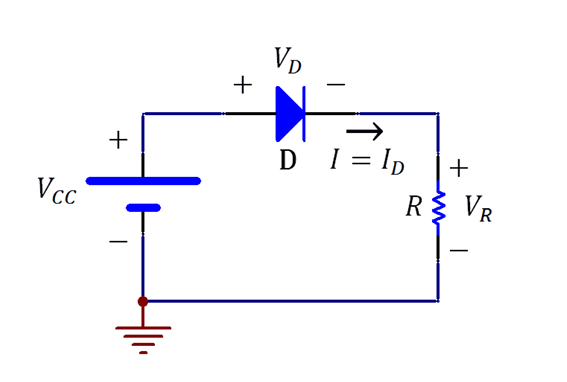
\includegraphics[width=0.48\textwidth]{circuito1.png} %las imagenes van en pdf
  \caption{Esquema de circuito de polarizacion directa de un diodo con resistencia en serie.}
  \label{fig:figura1}
  \end{figure}
%
    \begin{figure}[ht]
    \centering
    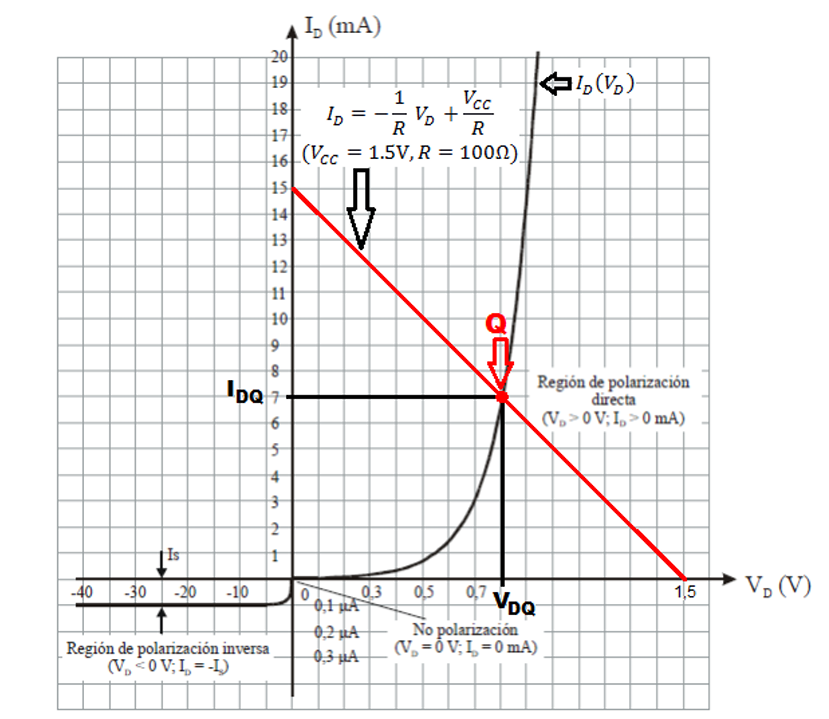
\includegraphics[width=0.48\textwidth]{curva-recta.png}
      \caption{Grafico de ejemplo de la curva caracteristica del diodo dada por ec(1) y una recta dada por ec(3) para un valor de $V_{CC}$ y $R$. 
      Punto Q es la interseccion de ambas curvas.}
  \label{fig:figura2}
  \end{figure}

%%
%
 
 
%Por la relacion entre la corriente y tension dada por ec(1) y ec(2), se puede determinar 
%la curva caracteristica del diodo, y a partir de esta, mediante ajuste no lineal, determinar $I_S$ y $\eta$,


Dado que la relación entre la corriente y tensión en el diodo está dada por la ec(1), y que la corriente y tensión
en el circuito están relacionadas por la ecuación de la recta dada por ec(3), se puede determinar la curva característica del diodo,
definiendo al conjunto de puntos $(I_D,V_D)$ que cumplen ambas ecuaciones, como puntos de trabajo o puntos Q. Por lo tanto, variando el voltaje de la fuente $V_{CC}$
 y la resistencia $R$, se pueden obtener diferentes puntos Q.
Si se aumenta o disminuye $V_{CC}$ para un mismo valor de R, se obtienen puntos Q obtenidos por intersecciones de rectas paralelas,
mientras que si se varían los valores de R para un mismo valor de $V_{CC}$, se obtienen puntos Q por intersecciones de rectas con diferente pendiente. Ver figura(2).
\section{METODOLOGÍA}
  %%
    \begin{figure}[ht]
    \centering
    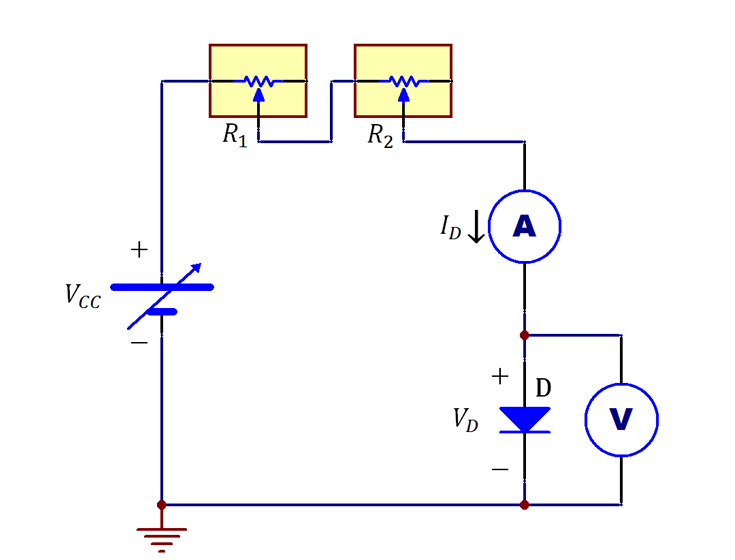
\includegraphics[width=0.48\textwidth]{circuito2.png} %las imagenes van en pdf 
    \caption{Esquema de circuito usado para las mediciones. $V_{CC}$ es la fuente,  $R_1$ y $R_2$ son reóstatos, $D$ es el diodo, A y V corresponden a amperímetro y voltímetro respectivamente.}
  \label{fig:figura3}
  \end{figure}

%%


Primero se debe verificar el correcto funcionamiento del diodo, para ello se lo conecta a un multímetro
en modo de prueba de diodos, y se revisa que la componente conduzca corriente en un sentido y no en el otro.


La temperatura ambiente del laboratorio se mide con un termómetro de mercurio, $T=(25.4\pm0.2)^\circ C=(298.6\pm0.2) K$.


Se disponen dos reóstatos, preferentemente uno de resistencia grande y otro de resistencia pequeña, en este caso $R_1=500\Omega$ y $R_2=25\Omega$, para
poder medir la curva característica del diodo en un amplio rango de voltajes y corrientes.


Luego se arma el circuito de la figura(2) con los elementos dados, y se conecta a la fuente de voltaje, estableciendo corriente máxima y voltaje $0V$.


Usando amperímetro en escala de $mA$ y voltímetro en escala de $V$, se miden los valores de corriente en el circuito y tensión en los extremos del diodo (por conexión corta),
variando la tensión de la fuente $V_{CC}$ en el rango de $0V$ a $4V$, usando la perilla de paso fino. Luego se toman mediciones con la fuente fija en $4V$ y
variando las resistencias $R_1$ y $R_2$ para obtener más puntos de la curva característica del diodo. Cuidando de nunca superar el límite de corriente configurada en el amperímetro.




Usando software de ajuste no lineal, se ajustan los puntos obtenidos a la ecuación de Shockley, usando funcion:
\begin{equation}y(x)=P_0 \left[e^{x/P_1}-1\right]\end{equation}
Donde $P_0$ y $P_1$ son los parámetros a ajustar, que corresponden a $I_S$ y $\eta V_T$ respectivamente.
\section{RESULTADOS}
Realizando el ajuste con ec(4) sobre los datos experimentales, ver figura(3), se obtienen los siguientes parámetros:
$$P_0=I_S=(1.0\pm0.1)10^{-8}A$$
$$P_1=\eta V_T=(4.41\pm0.03)10^{-2}V$$

%
   \begin{figure}[ht]
    \centering
    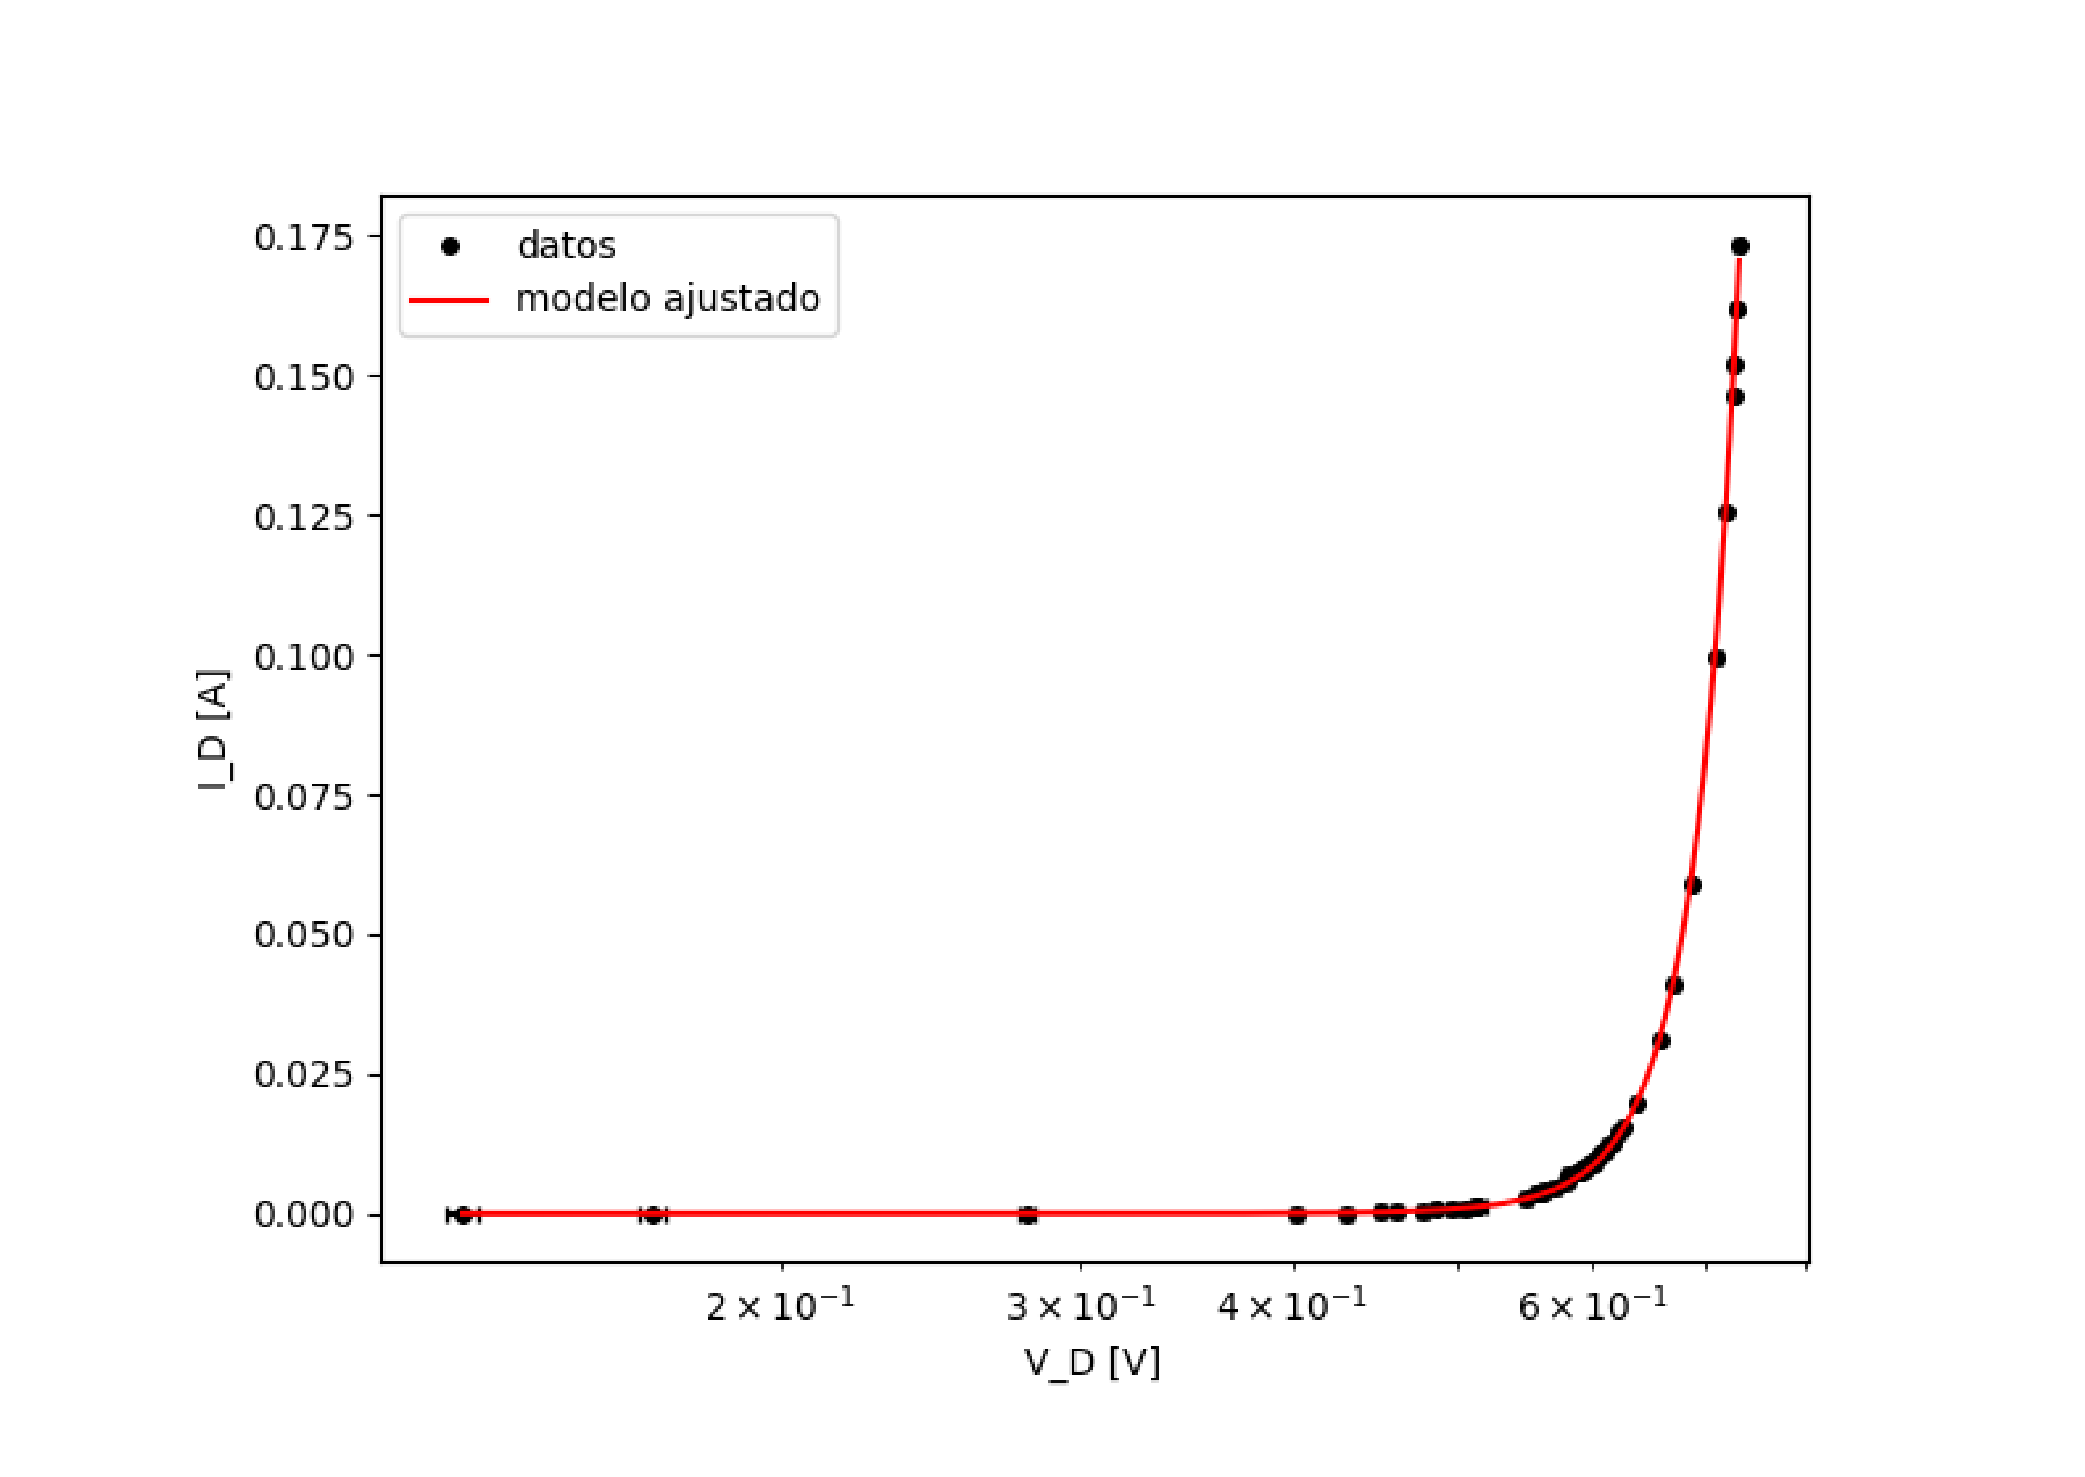
\includegraphics[width=0.48\textwidth]{ajuste.pdf} 
  \caption{Puntos experimentales de la curva característica del diodo, con sus respectivas barras de error, y ajuste no lineal a la ecuación de Shockley.}
  \label{fig:figura4}
  \end{figure}
  %%
  %
   \begin{figure}[ht]
    \centering
    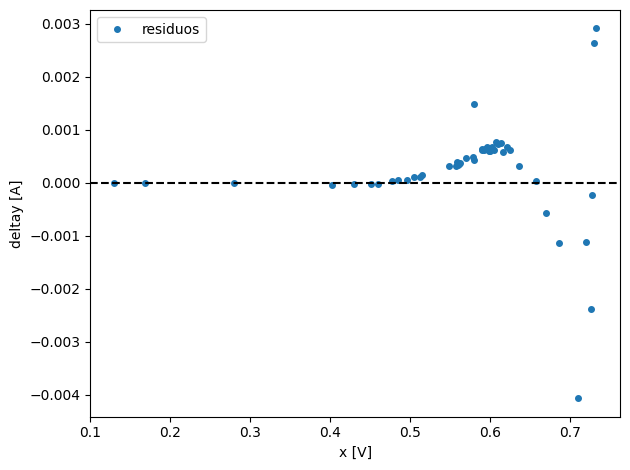
\includegraphics[width=0.48\textwidth]{residuo.png} 
  \caption{Gráfico de residuos del ajuste no lineal.}
  \label{fig:figura5}
  \end{figure}
  %%

Con la temperatura ambiente medida, se obtiene $V_T=(2.573\pm0.002)10^{-2}V$. Usando que $P_1=\eta V_T$, resulta $\eta=(1.71\pm0.01)$. Las incertezas las determino
por propagación de error.

\section{CONCLUSION}
Por figura(5) se puede observar que el ajuste no lineal a la ecuación de Shockley no es ideal, ya que los residuos  no se distribuyen aleatoriamente alrededor de cero,
mostrando un patrón sistemático, de modo que no describe completamente el comportamiento del diodo. Agregando un desfase a la ecuación de Shockley, no hubo cambio alguno
en los residuos, por lo que se podría concluir que el desfase no es un factor importante a considerar para mejorar el ajuste. Pudo haber afectado a las mediciones la resistencia
 en la conexión del diodo con el multímetro, provocando una caída de tensión no prevista, o el calentamiento del circuito tras varias horas de mediciones.


 Por la hoja de datos de diodo 1N5408, se sabe que a una temperatura ambiente de $25^\circ C$, el valor máximo de $I_S$ es de $5\times10^{-6}A$ , y dado que
la corriente inversa de saturación obtenido $I_S=(1.0\pm0.1)10^{-8}A$ está por debajo de este valor, se puede concluir que el diodo está funcionando correctamente.


Por otro lado, el valor de $\eta = (1.71\pm0.01)$
obtenido es consistente con el valor esperado para un diodo de silicio, que es del orden de 2 . Sin embargo, la temperatura del laboratorio (y del circuito) habría variado a lo largo
 de las mediciones, lo que podría haber afectado el valor de $V_T$ y por ende el valor de $\eta$ obtenido, lo que se podría mejorar en futuras mediciones
 controlando la temperatura ambiente, o tomando valor medio de varias temperaturas a diferentes horas.



\section{REFERENCIAS}
%\vspace{-3ex}%hace
1- Guia de laboratorio:“Trabajo de 
Laboratorio Nº4: Diodo”.
Facultad de Matemática, Astronomía, 
Física y Computación 2026. Aula virtual 
Física Experimental III 2026.


2- Manual Multimetro UNI-T UT39E+


3-  Hoja de Datos del diodo 1N5408, disponible en: \url{https://www.vishay.com}

\end{document}
